% !TEX root = ../main.tex

\chapter{绪论}


\section{引言}

编译器作为关键系统软件之一,其正确性对于计算机系统的安全运行有重要意义。
这是由于编译器可能在转换程序的过程中引入错误,导致目标程序的行为和源程序不一致,
进而使得在源程序端花费大量精力的测试和验证工作在目标程序层级失效。
虽然对于编译器一般会进行密集的测试,错误编译是小概率事件,但是这种偶发性的
由编译器引入的问题,对于安全关键系统而言是需要考虑的。
工业界长期以来对保障编译器正确性这个问题非常重视。例如,按照航空领域的RTCA DO178B/C标准~\cite{brosgol2010178c},
需要按照和机载软件一样的严格要求对待编译器。

对于庞大的编译器,通过测试找到它的错误其实是比较困难的。
编译器随机测试工具Csmith~\cite{csmith2011}已经发现了四百多个编译器错误,可见编译器中隐藏的风险数量之大。
编译器的形式化验证(Formal Verification)已被证实可以有效保证编译器的正确性,它从数学层面上确保了编译过程的正确性。
一个著名的例子是经过验证的C编译器CompCert~\cite{leroy2009formally},
它将C语言的一个有代表性的重要子集编译到了支持多种处理器架构的汇编代码(包括PowerPC、ARM、X86和RISC-V)。
其编译过程的正确性(即目标汇编程序保存了源C程序的语义)经过了形式化验证,并在Coq定理证明器中实现。
Csmith测试过的所有C语言编译器中,只有CompCert经过验证的部分是没有发现编译器错误的~\cite{csmith2011}。
在其他被测试的主流C语言编译器中间端都存在的错误,只有在CompCert中不存在。
并且,研究者们已经花费了大约六个CPU年去让Csmith寻找CompCert中的错误。
这样的结果有力地说明了,经过形式化验证的编译器在正确性和可靠性上具有重要地位。

CompCert已被应用于诸如核电站控制软件和飞行控制系统的开发。
清华大学王生原、尚书等人设计并实现了基于CompCert的L2C编译器~\cite{shang2017key},被用于安全关键的工业领域。
L2C的源语言是被广泛用于安全关键的工业领域(高铁、核电站等)的Lustre,
这些类型的应用对开发工具本身的安全性要求很高。它的目标语言是ComperCert中使用的C子集Clight。
南京大学冯新宇等人针对并发程序进行了单独编译验证~\cite{jiang2019towards}。他们提出了独立于语言的验证框架,
将顺序程序与无竞赛并发程序编译器验证工作联系起来,从而使针对顺序程序的编译器验证工作可以被重用。
使用这种框架,他们建立了CASCompCert。它扩展了ComperCert,可以对无竞赛Clight并发程序的单独编译进行验证,
且允许将并发Clight模块与包含良性竞赛的同步原语的x86-TSO实现进行连接。

延续传递风格(Continuation-Passing Style, CPS)是一种函数式程序的中间语言(Intermediate Representation, IR),
它明确了函数式程序的控制流,从而为程序基于控制流的分析和优化提供了便利。
延续传递风格的中间语言在函数式程序的编译器中被
广泛采用\cite{belanger-cpp2013,dargaye2009verification,zoe-oopsla2021,zoe-icfp2021,wang-esop2016}。
然而,这也意味着经验证的函数式编译器不能直接得到主流编译器基础设施(例如LLVM和GCC)的支持。
这些主流编译器基础设施采用静态单赋值(Static Single Assignment, SSA)形式的中间语言。 
SSA中间语言在工业编译器中大大流行,因为它可以通过强制让每个变量只能被赋值一次来实现
便捷而准确的数据流分析(Data-Flow Analysis, DFA),进而实现各种基于数据流分析的激进优化。
许多流行的命令式编程语言(例如Rust~\cite{balasubramanian2017system}和Swift~\cite{zhang2012swift})
使用这些编译器基础设施作为其后端,生成性能优越的代码~\cite{lattner2006introduction}。
一些工业级的函数式编译器也开始采用SSA形式的中间语言。例如,SML-New Jersey的
新版本已经将其后端转向了LLVM~\cite{farvardin2020new}。

在本文中,我们研究了如何构建基于SSA中间语言的经验证的函数式语言编译器。
具体而言,我们设计了从CPS到SSA的转换算法,并使用模拟技术对该转换过程的正确性进行形式化验证。
在经验证的编译器领域中将传统基于CPS的函数式编译器与基于SSA中间语言的主流编译器后端连接起来,
才能让高可靠函数式编译器复用基于SSA语言的编译器后端优化。
尽管研究人员已经探讨了CPS和SSA程序结构上的对应关系~\cite{appel1998ssa,ssabook}
和相互转换~\cite{farvardin2020new,kelsey1995correspondence},
但如何对转换算法进行形式化验证仍然是待解决的问题。

\section{主要贡献与章节安排}

本文的贡献总结如下:

\begin{itemize}
    \item
    我们的主要贡献是设计和验证了从CPS到SSA的转换算法。该转换过程的源语言是代表性的
    函数式语言PCF\cite{plotkin1977lcf},我们首先需要将其转换为CPS形式。
    转换算法的SSA目标语言是LLVM IR的一种简化版本,保留了LLVM IR的基本结构。
    该转换是基于CPS和SSA结构上的对应关系设计的~\cite{appel1998ssa,kelsey1995correspondence}。
    我们为PCF和SSA语言定义了小步操作语义,使用基于模拟的方法证明目标程序实现了
    源程序的语义保存。据我们所知,这是第一个经过验证的从CPS函数式程序到SSA的转换。
    
    \item 
    我们还利用该经验证的编译链构建了PCF语言的编译器原型。它是部分经过形式化验证的,
    为未来构建更复杂更完整的经验证函数式语言编译器打下基础。
    具体而言,我们首先实现并验证了直接风格PCF语言的CPS转换,并将它连接到经验证的CPS到SSA的编译过程。
    然后,我们通过Vellvm提供的抽象语法(Vellvm是一个经过验证的LLVM基础设施~\cite{zakowski2021modular}),
    将SSA中间语言转换为LLVM IR。
    
\end{itemize}

在本章接下来的内容中,我们在\ref{sec:background}节介绍了与此研究相关的背景知识,
包括函数式语言中的直接风格与延续传递风格表示形式、静态单赋值中间语言及其与延续传递风格的关系。
我们还简要介绍了程序语言的操作语义以及基于模拟技术的编译器形式化验证理论与框架。

在第\ref{ch:related}章中,我们讨论了领域内与本课题相关的工作,
包括一些经验证的函数式编译器和与静态单赋值中间语言有关的工作。
我们在第\ref{ch:trans}章中具体探讨了该编译过程的源语言与目标语言,并为它们提供了
小步操作语义。之后,我们设计并实现了从源语言到目标语言的编译算法,
并用示例程序展示了该算法的主要思想及工作过程。
在第\ref{ch:verify}章中,我们使用基于模拟的方法对该编译过程进行形式化验证。
我们首先对验证框架及步骤进行简要介绍,然后具体讨论了每一个编译步骤的前向模拟证明。
本文工作在Coq中的实现和评估将在第\ref{ch:implement}章中介绍。
在第\ref{sec:overview}节中,我们简要介绍了本文中构建的部分经验证的PCF编译器原型的各个组成部分。
之后,我们具体介绍了每一部分的代码实现,并评估了其工作量。
最后,我们在第\ref{ch:summary}章中对本文内容进行总结,并展望了基于该研究未来可继续开展的工作。

\section{相关背景} \label{sec:background}

在本节中,我们将对该课题的相关背景进行介绍。
本文工作涉及函数式编程、编译器常用中间语言形式以及编译器形式化验证方法等方向。
首先,我们会介绍函数式编程的概念及其特性。
然后,我们将说明CPS形式是如何帮助函数式程序显式地表示控制流的,
并介绍了静态单赋值中间语言的相关特性以及CPS和SSA结构之间的对应关系。
接下来,我们介绍了在经验证的编译器CompCert中提出的基于模拟技术进行编译器验证的框架~\cite{leroy2009formally}。

\subsection{函数式编程}

函数式编程(Functional Programming)是一种通过应用和组合函数来构建程序的编程范式,
也可以指实现这些编程范式的程序语言。
它以$\lambda$演算($\lambda$-Calculus)作为其数学基础~\cite{church1985calculi}。
在传统命令式编程中,计算通过执行程序语句序更新程序状态来实现。
相比之下,函数式编程中程序由包含函数定义和应用的表达式构成,而计算通过对表达式求值来实现。
函数式程序的一大特点是函数可以作为参数传递,或者被其他函数返回,形成所谓的高阶函数~\cite{sussman1998scheme}。
此外,函数式程序的执行不会引起改变程序状态的副作用(Side Effect),例如I/O、可变变量的赋值、指针重定向等。
函数式编程的基本宗旨就是纯粹的计算,程序执行的唯一效果就是产生计算结果。

这些特点使得函数式程序设计语言编写的程序更加简洁、安全和易于验证~\cite{hudak1989conception},
因此在并发编程、系统内存编程等方面获得了成功应用。
\begin{itemize}
    \item 函数式编程使程序在并发情况下表现出更简单的行为。
    如果对一个数据结构进行操作只会产生新的数据结构,而不会破坏旧结构的完整性,那么就不需要担心该结构的共享方式,
    因为程序一部分的更改不会破坏其另一部分所满足的不变式(Invariant)。
    在并发系统中,线程之间共享的可变状态是潜在的问题来源,所以这些因素非常关键。
    \item 函数式程序更容易进行并行化和物理上的分布式。如果运行程序进行计算除了产生结果外没有其他影响,那么在哪里运行它就无关紧要。
    同样,如果数据结构从不被破坏性地修改,那么它可以自由地在核或网络之间进行复制。
    实际上,大规模分布式查询处理器的核心Map-Reduce模式就是函数式编程的一个经典示例~\cite{chu2006map}。
    \item 如果一个过程或方法只是将输入映射到输出,而没有副作用,我们就可以把它看作是计算数学函数的具体方法。
    程序与简单的数学对象之间的直接联系支持形式化的正确性证明。
\end{itemize}

在学术界和工业界中,函数式编程的应用日趋广泛。
除了Haskell~\cite{o2008real}等纯函数式语言,OCaml、Erlang、Scala~\cite{cesarini2009erlang, odersky2014unifying}
等语言都对函数式编程有内生的支持,且诸多命令式编程语言如C++和Rust也在积极的引入函数式编程机制。
本文研究的函数式编程语言是学术界有广泛影响力的PCF(Programming Computable Functions)。
由于PCF可以看作是工业用函数式编程语言的核心,本文的研究结果可被推广至其他函数式语言。
关于PCF语言的更多特性将在第\ref{sec:cps}节中详述。

\subsection{延续传递风格} \label{sec:bg_cps}

函数式程序的表示形式有很多种,比如直接风格(Direct Style)和延续传递风格(CPS)。
图~\ref{cpsdirect}展示了同样含义的函数式程序在这两种不同表示风格下的例子。
CPS程序的关键特性在于通过延续(Continuation)明确地表示程序的控制流。
CPS中的延续指的是当前执行节点之后剩余需要计算的函数,
该函数把当前代码项计算得到的结果作为其输入。
具体来说,CPS函数需要将延续作为额外的参数传入,
当运行该函数得到计算结果后,程序就会通过调用该延续来传递这个值,也就是``返回''该结果。
以图~\ref{fig:cps2}为例,函数$h$在CPS中的延续参数为$k$,在得到最终结果$z$之后,
程序调用$(k\; z)$以返回$z$,并把$z$嵌入$k$所代表的剩余需计算的代码项。
当调用CPS函数时,调用者需要提供一个延续函数来表示剩余计算,且在CPS中所有中间结果、控制流中的控制点都需要被明确命名。
这些特点导致用户直接用CPS形式编写代码较为困难,但是由于明确表示的控制流利于程序分析和优化,
CPS是函数式语言编译器中常见的中间表示形式。

\begin{figure}
    % \vspace{-0.3cm}
    \centering
    \begin{subfigure}[b]{0.4\textwidth}
        \flushright
    % \small
     \begin{equation}
        \nonumber
        \begin{aligned}
        &  \mathbf{function}\; h(x,y) = \\
        & \quad (x*x)\; +\; (y*y) \\
        \end{aligned}
    \end{equation}
    \caption{直接风格}
        \label{fig:ori2}
    \end{subfigure}
 %   \hfill
    \begin{subfigure}[b]{0.5\textwidth}
        \flushleft
        % \small
        \begin{equation}
            \nonumber
            \begin{aligned}
            & \mathbf{function}\; h(x,y,k)= \\
            & \quad \mathbf{let}\; x_1=x*x\; \mathbf{in} \\
            & \quad\quad \mathbf{let}\; y_1=y*y\; \mathbf{in} \\
            & \quad\quad\quad \mathbf{let}\; z=x_1+y_1\; \mathbf{in}\; (k\; z) \\
            \end{aligned}
        \end{equation}
        \caption{CPS}
        \label{fig:cps2}
    \end{subfigure}
    \caption{直接风格和CPS形式的示例函数式程序}\label{cpsdirect}
  \end{figure}

CPS形式函数式程序的使用可以追溯到Scheme的编译器中~\cite{steele1978rabbit}。
之后,CPS形式的中间语言被应用到了SML-New Jersey编译器的基本框架中~\cite{shao1995type}。
为了利用CPS形式中间语言的优势,研究者们设计了多种将直接风格的函数式程序进行CPS转换的方法。
其中Plotkin的方法需要在后续进行管理性缩减(Administrative Reduction),以去除转换中产生的冗余$\lambda$结构~\cite{plotkin1977lcf}。
Felleisen等人提出了另一种方法非组合式的方法,其基于$\lambda$-演算的语义。
Danvy和Nielsen将这两种方法联系起来,可以只通过一步转换完成,不需要在后续过程中进行管理性缩减\cite{danvy2007one}。
Andrew根据对之前的研究者们关于CPS的工作的观察和总结,提出了特定的CPS语言规范~\cite{kennedy2007compiling}。
它适用于无类型的或有类型的函数式语言,并且可以表示循环、异常等。
这种CPS语言对函数和局部延续做了语法上的区分,后者总是可以被编译为跳转。
Andrew基于Standard ML语言的一部分演示了如何对函数式程序进行CPS转换。
他使用了Danvy和Nielsen的一步(One-Pass)CPS转换算法思想,把上下文作为参数,
让转换算法知道当前代码项被翻译之后会嵌入到哪里。

\subsection{静态单赋值} \label{sec:bg_ssa}

静态单赋值(SSA)是命令式语言编译器中一种广泛使用的中间语言类型。
在SSA中,每个变量只能在一处被赋值,且被使用之前必须已经被赋值。
这种性质很接近函数式语言中的名字绑定(Name Binding)~\cite{ssabook}。
变量被划分为不同的版本,新版本的变量往往使用原名加下标来表示,以使每个定义得到自己的版本。
$\phi$节点($\phi$-nodes)作为特殊的程序语句被插入到基本代码块的开头,
从而按照前驱基本块的名字生成新变量的赋值语句。
这样一来,变量的使用定义链(Use-def Chains)更加清晰,从而使许多编译器优化算法
在SSA中间语言上能够更好地实现,例如常量传播、无用代码消除、寄存器分配等~\cite{ssabook,kelsey1995correspondence}。
作为示例,图~\ref{ssacfg}展示了一个SSA程序的控制流图(Control-Flow Graph)。
其中,基本代码块$b_2$的前驱基本块可以是$b_1$或$b_2$本身。
不同的前驱基本块对变量$y$有不同的赋值,在$b_1$和$b_2$中变量$y$被赋予了不同版本的名称。
基本块$b_2$开头的$\phi$节点将$y_1$和$y_3$作为参数,根据执行时控制流的实际前驱基本块来
选择正确的版本赋值给新的变量$y_2$。

LLVM IR就是一种基于SSA的中间代码。它作为一种高层次的汇编语言,提供了编译系统的中间层,
使得不同语言可以相互连接起来,复用其后端优化~\cite{lattner2006introduction}。
除了LLVM,还有很多编译器是基于SSA的,例如GCC编译器的中间语言GIMPLE~\cite{callanan2007extending}、
面向微软.NET平台的即时编译中间语言CIL(Common Intermediate Language)~\cite{thai2003net}等。

\begin{figure}[htbp]
    \centering
    % \documentclass{article}
% \usepackage{tikz}
% \usetikzlibrary{chains,shadows.blur}

% \begin{document}
\begin{tikzpicture}[auto,
%   node distance = 12mm,
%   start chain = going right,
  box/.style = {draw,rounded corners,blur shadow,fill=white,
        align=center}]
 \small
 \node[box] (b1) at(0,0)    {$v_1 \leftarrow 1$\\ 
                    $z_1 \leftarrow 8$ \\ 
                    $y_1 \leftarrow 4$};      
 \node[box] (b2) at(3,0)    {$y_2 \leftarrow \phi(y_1,y_3)$\\
                    $x_1 \leftarrow 5 + y_2$ \\
                    $y_3 \leftarrow x_1 * z_1$ \\
                    $x_2 \leftarrow x_1 - 1$ \\
                    $\mathbf{if}\; x_2 = 0$};      
 \node[box] (b3) at(6.5,0)    {$w_1 \leftarrow v_1 +y_3$\\ 
                    $\mathbf{return}\; w_1$};  
 \node at(4.0,1.5) {false};
 \node at(4.8,0.3) {true};

 \coordinate (b1n) at ([yshift=-31] b1);
 \coordinate (b2n) at ([yshift=-43] b2);
 \coordinate (b3n) at ([yshift=-25] b3);

 \node at (b1n)  {$b_1$};
 \node at (b2n)  {$b_2$};
 \node at (b3n)  {$b_3$};
 
 \begin{scope}[rounded corners,-latex]
  \path (b2.60) edge[bend right=50] (b2.120)
        (b1) edge (b2) (b2) edge (b3) ;
%   \draw (b3.230) -- ++(0,-0.3) -| ([xshift=-5mm]b2.west) |-
%   ([yshift=3mm]b2.130) -- (b2.130);
 \end{scope}
\end{tikzpicture}
% \end{document}      
    \caption{SSA程序的控制流图示例}\label{ssacfg}
\end{figure}

Appel等人~\cite{appel1998ssa}发现SSA也是一种函数式语言:$\lambda$演算和SSA虽然有不同的形式,
但它们所做的工作其实是相同的。
L. Beringer~\cite{ssabook}给出了SSA的函数式表示,
将SSA中的相关术语与函数式编程中的概念联系起来。
例如,函数式语言中的$let$绑定对应着SSA中的赋值、绑定变量(Bound Variable)的词法作用域
(Lexical Scope)对应着SSA中的可支配区域(Dominance Region)。
$let$绑定与变量定义点之间的对应关系还延续到了程序结构的其他方面。
与命令式语言中的返回地址或函数指针相似,延续指定了当前代码片段求值完成后程序下一步该如何执行。
SSA中的控制流图对应着函数式编程中的函数,虽然顶层延续的参数在控制流图中并不是明确可见的,
但它对应一个命令式调用中用来保存返回地址的地方。

事实上,SSA和CPS都是通过强制执行特定的命名规则,在语法层面上明确表示出程序结构的某个方面。
这样,编译器就可以更加方便地对程序进行分析和处理。
在CPS形式的函数式程序中,延续的形参恰好起到了$\phi$函数的作用:统一来自各个调用点的变量名称,
这个名称将在之后的代码中被使用。并且,CPS程序中绑定的变量名的范围和SSA程序中变量的可支配区域
都在函数调用或跳转到控制流合并点时终止。从这一事实来看,CPS程序其实已经有了SSA程序基本结构。

Kelsey~\cite{kelsey1995correspondence}通过将CPS中的$\lambda$进行标注来区分完整过程、跳转、延续,
进而将被这种标注的CPS程序转换为一种SSA程序。然而,Kelsey工作中采用的的CPS和SSA语言与本文中所使用的差距较大。
Kelsey工作中的CPS语言将二元表达式的参数和条件语句中的条件视为表达式,使其更类似于带有延续元素的标准函数式程序。
例如,在Kelsey的工作中,表达式$k\; ((x+y)+z)$是被允许的,但在我们的工作中,
它必须转换为
$\mathbf{letop}\; x_0 = x+y\; \mathbf{in}\; (\mathbf{letop}\; x_1 = x_0+z\; \mathbf{in}\; k\; x_1)$。
此外,Kelsey的转换算法选择先合并CPS过程,然后再将其作为一个整体进行转换。
这样一来,SSA程序的顶层单元是一整个过程,没有函数调用,这与本文中使用的基于LLVM IR的SSA语言不同。

\subsection{小步操作语义} \label{sec:smallop}

为了对编译算法的正确性进行验证,首先需要将程序与其运算过程用形式化的方法联系起来。
接下来我们将介绍对程序代码项的求值过程进行精确定义的方法,即定义程序的语义。
形式化定义的程序语义可以分为三种基本的类型:操作语义(Operational Semantics)、
指称语义(Denotational Semantics)和公理语义(Axiomatic Semantics)\cite{pierce2002types}。

\begin{itemize}
    \item 公理语义不是去另外定义程序的行为,而是把规则本身作为语言的定义,即代码项本身的含义就是可以被证明的东西。
    \item 指称语义比较抽象,它将代码项视作一些数学对象,比如数字和函数。
    找到指称语义需要找到语义域(Semantic Domains)的集合,然后定义解释函数
    (Interpretation Function),将代码项映射到语义域元素中。
    \item 操作语义是通过直接描述程序执行时行为来定义语义的,而不是像指称语义那样给其附加数学意义。
    为了描述程序的行为,操作语义为程序语言定义了一个简单的抽象机器(Abstract Machine),
    程序的状态是它的代码项和一些附加信息内容。对于程序的每一个状态来说,
    要么可以通过对代码项进行化简得到下一个状态,要么宣告机器停机。
    对于这个抽象机器来说,它的机器代码就是该程序语言,而不是真实机器所用的微处理器指令集。
    操作语义将程序描述为一系列的计算步骤。对于函数式程序,会终止的计算序列在最后一步返回程序的值。
\end{itemize}

操作语义分为大步操作语义和小步操作语义。大步语义描述程序执行的整体结果,
小步语义则描述一个执行计算步骤。大步语义描述的下一个状态往往需要多个小步语义转换步骤实现。
大步操作语义则更加接近人类对程序运行自然的理解,也被称为自然语义。
但是,大步操作语义有一定局限性。例如,它不能描述并发编程中程序执行的中间状态,
而这些状态应当可以被同时执行的代码观察到~\cite{pierce2010software}。
本文中使用的是小步操作语义(Small-Step Operational Semantics)。

使用$\rightarrow $表示一步计算步骤,它是程序状态之间最小的二元关系。
使用$\xrightarrow{*} $表示多步计算步骤,即一步计算的自反传递闭包。
那么,以简单的布尔值条件语句为例,它的小步语义和大步语义区别如图\ref{fig:bigsmall}。

可以看到,在小步操作语义中,语义规则可以分为计算型规则(Computation Rules)
和聚合型规则(Congruence Rule)。S\_If\_True和S\_If\_False属于计算型规则。
S\_If\_True意为,如果条件代码项的值是true,表达式可以经过一步转换变为$t_2$代码项。
同理,S\_If\_False规则表示在条件为false时转换到$t_3$。
S\_If则属于聚合型规则,意为如果$t_1$经过一步转换步骤变为$t'_1$,
那么整个条件语句会变成条件为$t'_1$的代码项。它并没有做真正的求值工作,没有决定程序下一步向哪个分支走,
但是它告诉了程序应当先去对条件语句的哪个部分进行进一步计算。
如果没有S\_If的帮助,我们就无法知道$t_1$、$t_2$和$t_3$中要先对谁求值。
B\_If\_True说明如果$t_1$经过若干步求值可以化简为true,那么下一个状态转换到代码项$t_2$。
B\_If\_False则相反。

一种语言可以有多种不同的操作语义,即有不同的抽象机器。它们在执行同一程序时,最终产生的行为是一致的。
对于不同的语言,证明它们的操作语义定义的抽象机器在执行某一程序及其转换后得到的程序时的行为是一致的,
则证明了转换过程的正确性。

\begin{figure}[htbp]
    \vspace{13pt}
    \centering
    \begin{subfigure}[b]{0.8\textwidth}
        条件表达式示例语法:
        \begin{align*}
        v\, := &\,  true\; |\; false \\
        t\, := & \, v\; |\; \mathbf{if}\; t\; \mathbf{then}\; t\; \mathbf{else}\; t
        \end{align*}
    \end{subfigure}
    \vfill
    \begin{subfigure}[b]{0.8\textwidth}
        小步操作语义:
    \begin{equation}
        \setlength{\jot}{10pt}
        \nonumber
            \begin{aligned}
            & \text{S\_If\_True} \qquad \mathbf{if}\; true\; \mathbf{then}\; t_2\; \mathbf{else}\; t_3\rightarrow t_2 \\
            &  \text{S\_If\_False} \qquad \mathbf{if}\; false\; \mathbf{then}\; t_2\; \mathbf{else}\; t_3\rightarrow t_3 \\
            & \text{S\_If} \qquad \displaystyle{\frac{t_1\rightarrow t'_1}{\mathbf{if}\; t_1\; \mathbf{then}\; t_2\; \mathbf{else}\; t_3\rightarrow \mathbf{if}\; t'_1\; \mathbf{then}\; t_2\; \mathbf{else}\; t_3 }}
        \end{aligned}
    \end{equation}
      大步操作语义:
        \begin{equation}
            \setlength{\jot}{10pt}
            \nonumber
            \begin{aligned}
                & \text{B\_If\_True} \qquad \displaystyle{\frac{t_1\xrightarrow{*} true\quad t_2\xrightarrow{*} v_2}{\mathbf{if}\, t_1\, \mathbf{then}\, t_2\, \mathbf{else}\, t_3\xrightarrow{*} v_2 }} \\       
                & \text{B\_If\_False} \qquad \displaystyle{\frac{t_1\xrightarrow{*} false\quad t_3\xrightarrow{*} v_3}{\mathbf{if}\, t_1\, \mathbf{then}\, t_2\, \mathbf{else}\, t_3\xrightarrow{*} v_3 }}
            \end{aligned}
        \end{equation}
    \end{subfigure}
    \vspace{5pt}
    \caption{小步操作语义与大步操作语义区别示例}\label{fig:bigsmall}
\end{figure}


\subsection{编译器形式化验证} \label{sec:compcertbackend}

我们使用CompCert~\cite{leroy2009formally}基于模拟(Simulation)技术的形式化验证框架来证明转换过程的正确性。
经过形式化验证的C语言子集编译器CompCert是由INRIA的Xavier Leroy领导开发的,在Coq定理证明工具中实现。

CompCert提供了一套基于模拟技术验证编译过程正确性的理论和框架。该框架将编译过程的正确性定义为
语义保存性质(Semantic Preservation Property),即目标程序的行为应该与源程序的行为一致。
我们将程序的行为(Behaviors)描述为由小步操作语义生成的轨迹(Trace),
以便直接推导出编译器的正确性证明。根据CompCert中对语义保存性质的讨论,
通过为安全的源程序建立后向模拟(Backward Simulaion),可以证明语义保存性质。

接下来,我们会介绍一些概念来说明什么是安全程序的后向模拟。
通过程序语言的语义将可观察行为(Observable Behaviors)与程序关联起来,
可以把程序的可观察行为分为终止(Termination)、发散(Divergence)和出错(Going wrong)。
如果用$P_1$表示源程序,$B$表示可观察行为,那么$P_1 \Downarrow B$表示执行程序$P_1$获得的可观察行为为$B$。
同样的表示方法也可以应用于目标程序。在CompCert框架中,仅对不会出错的安全的源程序提供正确性保证。
如果我们将编译过程表示为$\mathcal{T}$函数,则经过转换得到的目标程序可以表示为$\mathcal{T}(P_1)$。

最严格的语义保存性质被记为安全程序的\textbf{双向模拟},即源程序和目标程序有完全一致的行为。
对于安全程序$P_1$和可观测行为$B$,
\begin{equation}
    P_1 \Downarrow B \Longleftrightarrow \mathcal{T}(P_1) \Downarrow B.
\end{equation}
双向模拟在大多数情况下过于严格。如果源程序不是确定性的,其实编译器应该被允许选择其中一种可能的行为。
这样一来,我们可以将编译安全程序的正确性描述为:目标程序的行为是可接受的源程序行为。
那么,安全源程序的\textbf{后向模拟}可以表示为:如果$P_1$是一个安全程序,
则对于所有的可观察行为$B$,
\begin{equation}
    \mathcal{T}(P_1) \Downarrow B \Longrightarrow P_1 \Downarrow B.
\end{equation}
然而,直接证明后向模拟是比较困难的。可以先建立从安全源程序到目标程序的前向模拟(Forward Simulation),
再根据目标程序的确定性和前向模拟来推导出后向模拟。这些不同的语义保存性质之间的关系如图\ref{fig:relation}所示。
安全源程序的\textbf{前向模拟}可以表示为:如果$P_1$是一个安全程序,则对于所有的$B$,
\begin{equation}
P_1 \Downarrow B \Longrightarrow \mathcal{T}(P_1) \Downarrow B.
\end{equation}
虽然前向模拟成立的情况下目标程序也可能有源程序不可接受的多余行为,
但是在目标程序具有确定性的情况下无需考虑这样的问题。
由于目标程序是确定性的(Deterministic),它只与一种行为相关联。
因此,目标程序不会具有$P_1$没有的额外行为。在这种情况下,可以从前向模拟中导出安全程序的后向模拟。

\begin{figure}[htbp]
    \centering
    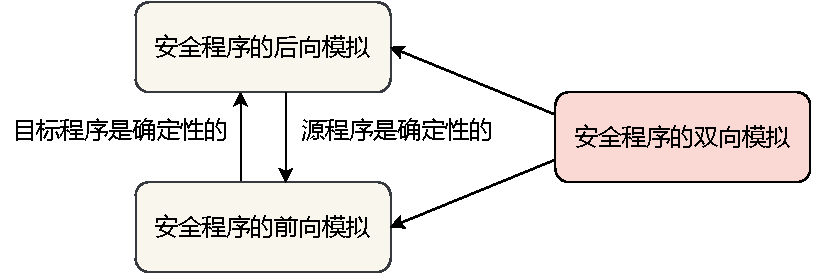
\includegraphics[width=0.7\linewidth]{figures/relation.pdf}
    \caption{语义保存性质关系}\label{fig:relation}
\end{figure}

为了证明源语言$L_1$转换为目标语言$L_2$的编译过程满足前向模拟性质,
关键在于建立程序状态$S_1$和$S_2$之间的不变式(Invariant)$S_1\sim S_2$,
并证明它在源程序和目标程序的执行过程中始终成立。
按照CompCert的方法,我们首先需要为$L_1$和$L_2$定义操作语义。
对于任何源程序$P_1$和目标程序$P_2$,我们需要证明$P_1$和$P_2$的初始状态满足不变量$\sim$。
然后,我们需要证明它们的内部执行步骤始终可以通过$\sim$相关联。
也就是说,假设$S_1\sim S_2$,源程序的状态在一步执行后从$S_1$转换到$S'_1$,
那么目标程序状态从$S_2$转换到某个$S'_2$,需要保证在转换后$S'_1\sim S'_2$成立。
根据从$S_2$到$S'_2$的转换步骤数量,可以将模拟图(Simulation Diagram)分为以下几种:

\begin{figure}[ht]
    % \vspace{-10pt}
    \centering
    \begin{subfigure}[b]{0.3\textwidth}
        % \flushleft
        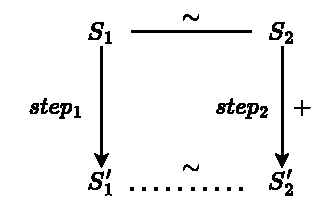
\includegraphics[width=1\linewidth]{figures/plusstep.pdf}
        \caption{多步模拟}
        \label{fig:plus}
    \end{subfigure}
    \begin{subfigure}[b]{0.6\textwidth}
        % \flushright
        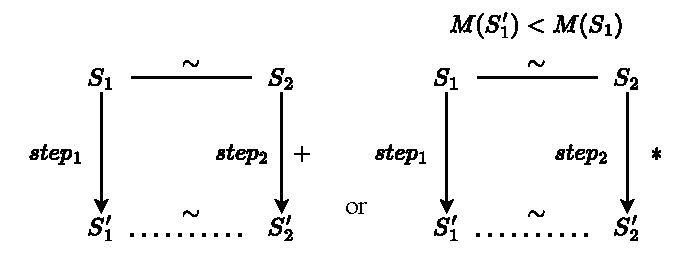
\includegraphics[width=1\linewidth]{figures/starstep2.pdf}
        \caption{星形模拟}
        \label{fig:star}
    \end{subfigure}
    \caption{不同类型的模拟图}\label{simustep}
\end{figure}

\begin{itemize}
    \item 一步模拟(Lock-Step Simulation)表示$S_2$经过一步转换到达$S'_2$状态。
        然而,对于大多数转换算法来说,一步模拟的前提要求太严格了,我们需要对其进行放宽。
    \item 多步模拟(Plus Simulation)表示$S_2$经过一步或多步转换到达$S'_2$(如图~\ref{fig:plus})。
        有时,从$S_1$到$S'_1$的转换对于状态$S_2$没有任何影响,比如删除冗余代码。
        因此,在某些情况下,多步模拟的条件也需要放松。
    \item 星形模拟(Star Simulation)表示$S_2$经过零步或一步或多步转换到达$S'_2$状态(如图~\ref{fig:star})。
        在这种条件下,可能会出现一种违反语义保存性质的情况:源程序发散,而目标程序保持在$S_2$状态,
        它们之间的状态仍然始终满足$\sim$不变式。为了防止出现这种``无限驻留''问题,我们需要
        为源程序的状态定义一个度量函数$M$,它随着源程序的执行过程严格减小。
        增添了度量函数$M$相关的限制,我们就能通过模拟保存源程序的发散行为了。
\end{itemize}

正如我们将在第~\ref{ch:verify}章中讨论的那样,CPS转换的前向模拟满足多步模拟性质,
而对于CPS到SSA的转换,我们需要使用星形模拟。根据上述模拟图性质以及
源程序和目标程序初始状态的对应关系,我们可以推导出安全程序的前向模拟。
结合目标语言的确定性,即可推导出安全程序的后向模拟。

由于语义保存性质具有可组合传递(Transitively Composable)的性质,
我们可以先分别证明各个编译过程的语义保存性质,然后将证明得到的定理组合起来推导出整个编译过程的正确性。
例如,如果编译过程$\mathcal{T}$被分解为两个转换阶段$\mathcal{T}_1$和$\mathcal{T}_2$,
$\mathcal{T}$可以被视为它们的组合。对于一个安全的程序$P$,如果没有发生编译时错误(Compiler-Time Error),
$\mathcal{T}(P) = \mathcal{T}_2(\mathcal{T}_1(P))$。
如果我们可以验证$\mathcal{T}_1$和$\mathcal{T}_2$的正确性,那么$\mathcal{T}$也得到了验证。

